% ICSE 2027 Research Track — submission draft
% TODO: anonymize self-citations before 2026-06-30 (see docs/cfp.txt)
% TODO: confirm PC conflict-of-interest rules (todo.md)

\documentclass[10pt,conference]{IEEEtran}

\usepackage[T1]{fontenc}
\usepackage{lmodern}
\usepackage{microtype}
\usepackage{booktabs}
\usepackage{array}
\usepackage{graphicx}
\usepackage{amsmath}
\usepackage{amssymb}
\usepackage{xcolor}
\usepackage{tikz}
\usetikzlibrary{arrows.meta,positioning,calc,fit,backgrounds}
\usepackage[hidelinks]{hyperref}
\usepackage{url}

% --- discourage single lines at page tops/bottoms
\widowpenalty=10000
\clubpenalty=10000

\begin{document}

% TODO: name the artifact. Working names: PowerMag / CompoMag / StakeMag.
% See docs/research-plan.md and todo.md for the decision.
\title{Beyond Cognition: Organizational-Power Personas for Stakeholder-Aware Evaluation of AI-for-SE Tools}

% Double-anonymous: leave authors blank.
\author{}

\maketitle

%==============================================================
\begin{abstract}
%==============================================================
AI-for-software-engineering (AI4SE) tools are increasingly evaluated on
internal metrics (coupling, cohesion, accuracy, F1, win-tie-loss) that assume
the ``What'' of a generated artifact can be assessed the moment it is
created. This assumption holds for chess and vision, the canonical domains of
Sutton's Bitter Lesson. It does not hold for software engineering, where
reliability, maintainability, and value-fit emerge slowly and depend on
\emph{which} stakeholder is asking. Prior persona-based evaluations (notably
the GenderMag framework and its recent SE extensions) partly acknowledge
this, but use a small fixed cast of cognitive personas that does not vary by
organizational power or time horizon.

This paper extends the five cognitive facets of GenderMag with two
organizational-power axes (\textsf{Control} and \textsf{Now}) distilled from
Boehm-style stakeholder analyses, producing a composite seven-facet persona
space that is generated rather than enumerated. We show that (a) LLM-simulated
personas drawn from this space are behaviorally distinguishable by an
independent LLM-as-Judge, with axis-level recovery above chance, and (b) on
the MOOT optimization benchmark, the extension surfaces at least one
stakeholder flip---a case where cognitive-only personas agree on a tool
recommendation while the composite personas disagree along the new power
axes. Our contribution is a named, open-source persona generator plus the
validation protocol we apply to it, both available at
\textsf{[redacted for review]}.
\end{abstract}

%==============================================================
\section{Introduction}
%==============================================================

% --- Paragraph 1: everyone does X
It is now routine in software engineering research to evaluate an automated
tool---a defect predictor, an architecture recommender, a code synthesizer,
an explainability module---by reporting its score on an internal metric
(accuracy, F1, coupling, cohesion, win-tie-loss). The AI4SE literature has
standardized this practice across a dozen subfields, and the latest wave of
LLM-based tools has amplified rather than challenged it.

% --- Paragraph 2: X has a problem
Sadly, the internal-metric stance has a hidden assumption that does not
survive contact with real software organizations. Every canonical
AI-success story cited in favour of scaling---chess, Go, vision,
speech---shares a quiet property: \emph{the ``What'' of a generated output
can be assessed the moment it is created}. A move is good or bad in
milliseconds; a label matches ground truth immediately; a phoneme aligns or
does not. Software engineering has no such oracle. Reliability emerges 18
months into production. Maintainability is measured by whoever inherits the
code. Value-fit is measured against a stakeholder's goals, which may
themselves shift. Recent empirical work makes the disconnect concrete: on
industrial legacy systems, automated tool outputs rated ``optimal'' by
internal metrics are rejected by maintainers whose profiles emphasize
different granularity preferences~\cite{carvalho2024usefulness}.

% --- Prior-work throw
Persona-based evaluation is the community's partial response to this gap.
The GenderMag framework~\cite{burnett2016gendermag} operationalizes five
cognitive facets (motivations, information-processing style, computer
self-efficacy, risk attitude, learning style) into three canonical personas
(Abi, Pat, Tim) and has been applied in over 200 software usability studies.
Recent work extends this to AI-for-SE by crossing GenderMag profiles with
three software-team roles, yielding nine personas and a validated LLM-as-Judge
protocol for behavioral distinguishability~\cite{estes2026se4ai}. But these
casts are small, categorical, and---by design---\emph{cognitively} oriented.
Their own authors flag the limit: role-constraint already suppresses
cognitive-style signals, which suggests that a single role axis
under-represents the space of stakeholder variation that actually matters for
SE tool adoption.

% --- Paragraph 3: the insight
The insight we offer here is that \emph{the missing dimension is
organizational power}, not a richer cognition model. A junior developer and
a chief architect may share every cognitive facet yet disagree sharply on
tool recommendations, because their positions in the organization dictate
different time horizons, different acceptable risks, and different
accountability. Boehm-style stakeholder analysis has long modelled these as
four orthogonal axes (\textsf{Now}, \textsf{Build}, \textsf{Change},
\textsf{Control})~\cite{boehm2004valuebased,menzies2009value}, but that
vocabulary has not been ported into the cognitive-persona literature. We
port it. The result is a seven-facet persona space---five cognitive, two
positional---in which personas are \emph{generated} as weighted mixes of
canonical stakeholder groups rather than enumerated as a fixed cast.

% --- Paragraph 4: what we did, + contributions
Concretely, this paper contributes:
\begin{itemize}
  \item A composite seven-facet persona model (§\ref{sec:model}) that
    unifies GenderMag's cognitive facets with two organizational-power axes
    derived from Boehm-style stakeholder analysis, formalized so that
    personas can be generated automatically as weighted mixes of eight
    canonical stakeholder groups.
  \item A validation protocol (§\ref{sec:method}) extending the LLM-as-Judge
    methodology of~\cite{estes2026se4ai} to seven facets, with rubric scoring
    and blind classification under Krippendorff-$\alpha \ge 0.80$ and
    Cohen-$\kappa \ge 0.61$ reliability thresholds.
  \item An empirical demonstration (§\ref{sec:results}) on the MOOT
    optimization benchmark~\cite{menzies2025moot} that (a) the composite
    personas are behaviorally distinguishable along the two new axes
    (\textbf{RQ1}), and (b) the composite model reveals a tool-evaluation
    flip case invisible under GenderMag-only personas (\textbf{RQ2}).
  \item An open-source persona generator and replication package
    (\textsf{[redacted for review]}).
\end{itemize}

% --- Digressions / CYA
Before proceeding we clarify two points. First, we do not claim the composite
model is \emph{complete}: seven facets are demonstrably more than five but do
not exhaust the space of stakeholder variation (e.g., organizational culture,
regulatory regime, and accountability depth are out of scope here).
Second, following~\cite{estes2026se4ai} we simulate stakeholders with LLMs
rather than recruiting human participants, inheriting the empirical
equivalence argument of~\cite{schuller2024personas}; we treat this as a
load-bearing assumption and return to it in the threats section
(§\ref{sec:ttv}).

%==============================================================
\section{Background and Related Work}
\label{sec:background}
%==============================================================

\subsection{The decades-old complaint}
The tension between internal-metric evaluation and stakeholder-conditioned
evaluation is not new. Brooks's V-diagram~\cite{brooks1976mythical} already
argued that the code is not the primary artifact of a software project;
\emph{what was learned} while building it is. Swartout's XPLAIN
system~\cite{swartout1983xplain} showed that systems generated without
preserving the \emph{Why} cannot justify themselves to users. Boehm's
value-based software engineering keynote~\cite{boehm2004valuebased}
explicitly called for SE-tool assessment by stakeholder value rather than
functionality alone. These observations form a consistent thread: SE artifacts
derive meaning from context, and any evaluation that abstracts that context
away is evaluating the wrong thing.

\subsection{The twin stakeholder-conditioning result}
Two papers, fifteen years apart, make the complaint empirically concrete.
Menzies and colleagues~\cite{menzies2009value} apply AI search to the
standard COCOMO/COQUALMO models under two different value functions
(``better, faster, cheaper'' versus risk-exposure) and report that
\emph{``if one value function approves of an action then the other usually
approves of not that action''}. Carvalho et al.~\cite{carvalho2024usefulness}
apply search-based microservice identification to an industrial Java system
and find that the same automatically-generated architecture is rated
``adoptable'' by fine-grained-preferring maintainers and ``not adoptable'' by
coarse-grained-preferring ones. One finding at the level of project values,
one at the level of maintainer preferences. Both reject universal-claim
evaluation. Both call for interactive, stakeholder-conditioned methods.

\subsection{Persona-based methods and their limits}
The methodological response in the SE community has been persona-based
walkthrough and simulation. GenderMag~\cite{burnett2016gendermag} derives
five cognitive facets from gender-difference research in HCI, instantiated as
three canonical personas (Abi, Pat, Tim). More recent work extends GenderMag
with software team roles and uses LLMs to simulate persona
responses~\cite{estes2026se4ai}, validating behavioral consistency through a
two-judge LLM-as-Judge protocol with rubric scoring and blind classification.
This line has matured into a reproducible methodology, but it inherits a
structural limit: the persona cast is small, fixed, and cognitively oriented,
and the single role axis compresses the organizational-position dimension
into a single gradient of technical depth.

\subsection{Stakeholder analysis and value-based SE}
Independently of the persona line, value-based
SE~\cite{boehm2004valuebased,biffl2005vbse} and stakeholder-aware decision
support~\cite{menzies2009value} have developed a vocabulary for
organizational position that the persona line has not absorbed: time horizon
(\textsf{Now}), consumption versus production (\textsf{Build}), appetite for
change (\textsf{Change}), and organizational authority (\textsf{Control}). In
this formulation, an organization is a weighted mix of stakeholder groups
(users, customers, developers, QA, managers, executives, regulators, ops),
and each candidate action has both objective consequences (cost, effort,
defect count) and a distribution of social consequences across the
stakeholder mix.

% --- Related-work throw
\subsection*{In summary}
Prior work has either (a) modelled stakeholders cognitively with small fixed
persona casts~\cite{burnett2016gendermag,estes2026se4ai}, or (b) modelled
stakeholders positionally with group-level value analyses that never made it
into persona-based tool
evaluation~\cite{boehm2004valuebased,menzies2009value}. For the rest of this
paper we explore a composite that unifies the two and is automatically
generated rather than enumerated, and we test whether the composite reveals
stakeholder flips invisible under cognitive-only personas.

%==============================================================
\section{A Composite Persona Model}
\label{sec:model}
%==============================================================

% --- Page-2 "groovy graphic" lives here.
\begin{figure*}[t]
  \centering
  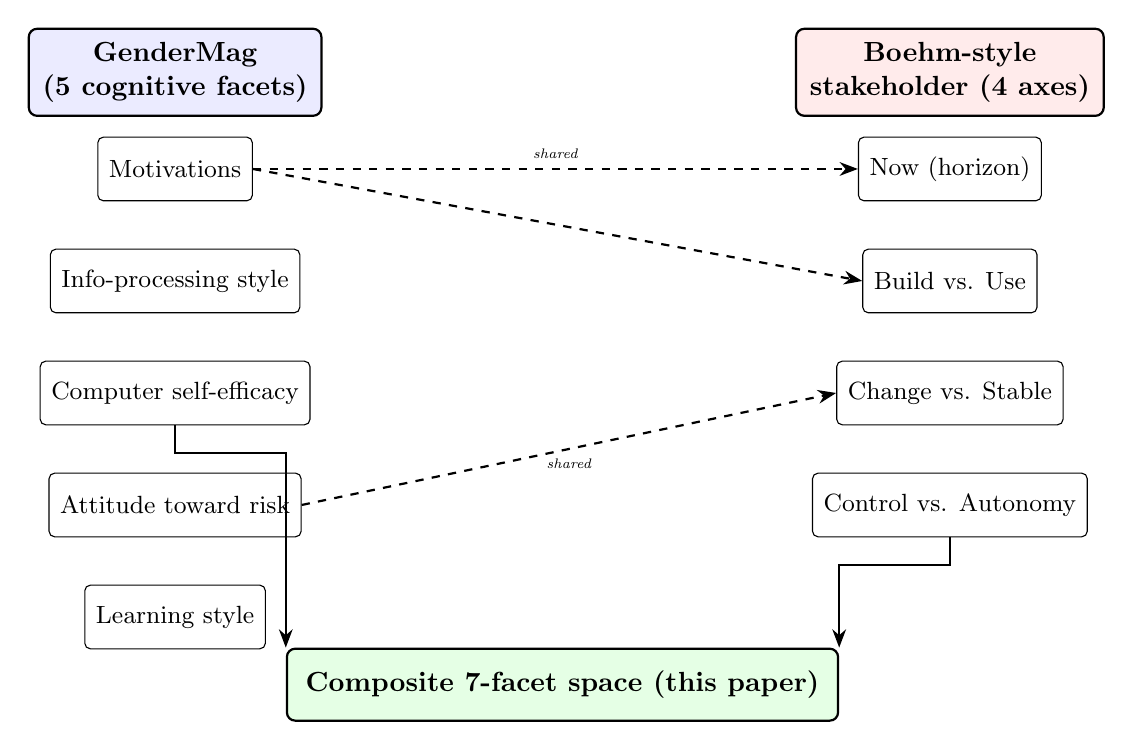
\begin{tikzpicture}[
    >=Stealth, node distance=0.6cm,
    every node/.style={font=\small},
    fac/.style={draw, rounded corners=2pt, align=center, inner sep=4pt, minimum height=2.3em},
    hdr/.style={draw, thick, rounded corners=3pt, align=center, inner sep=5pt, minimum height=2.6em, font=\bfseries},
    arr/.style={->, thick}
  ]
    \node[hdr, fill=blue!8] (cog) {GenderMag\\(5 cognitive facets)};
    \node[fac, below=0.25cm of cog] (c1) {Motivations};
    \node[fac, below=of c1]          (c2) {Info-processing style};
    \node[fac, below=of c2]          (c3) {Computer self-efficacy};
    \node[fac, below=of c3]          (c4) {Attitude toward risk};
    \node[fac, below=of c4]          (c5) {Learning style};

    \node[hdr, fill=red!8, right=6cm of cog] (org) {Boehm-style\\stakeholder (4 axes)};
    \node[fac, below=0.25cm of org] (o1) {Now (horizon)};
    \node[fac, below=of o1]          (o2) {Build vs. Use};
    \node[fac, below=of o2]          (o3) {Change vs. Stable};
    \node[fac, below=of o3]          (o4) {Control vs. Autonomy};

    \node[hdr, fill=green!10, below=1.1cm of $(c5)!0.5!(o4)$, minimum width=7cm] (comp) {Composite 7-facet space (this paper)};

    % overlap arrows
    \draw[arr, thick, dashed] (c1.east) -- node[above, pos=0.5, font=\tiny\itshape]{shared} (o1.west);
    \draw[arr, thick, dashed] (c1.east) -- (o2.west);
    \draw[arr, thick, dashed] (c4.east) -- node[below, pos=0.5, font=\tiny\itshape]{shared} (o3.west);

    % inclusion into composite
    \draw[arr] (c3.south) -- ++(0,-0.35) -| (comp.north west);
    \draw[arr] (o4.south) -- ++(0,-0.35) -| (comp.north east);

  \end{tikzpicture}
  \caption{The composite persona space unifies GenderMag's five cognitive
  facets~\cite{burnett2016gendermag} with Boehm-style stakeholder
  axes~\cite{boehm2004valuebased,menzies2009value}. Two dimensions are
  independently identified by both frameworks (\emph{motivations} and
  \emph{risk attitude}); three are cognitive-only; two are positional-only.}
  \label{fig:composite}
\end{figure*}

% TODO: flesh out — pull more detail from docs/background.md and docs/validation-plan.md

\subsection{Facets}
We combine five cognitive facets~\cite{burnett2016gendermag} with two
organizational-power facets drawn from Boehm-style stakeholder
analysis~\cite{boehm2004valuebased,menzies2009value}:

\begin{enumerate}
  \item \textsf{Motivations} --- task-oriented vs. technology-oriented.
  \item \textsf{Information processing} --- comprehensive vs. selective.
  \item \textsf{Self-efficacy} --- low / medium / high.
  \item \textsf{Risk attitude} --- risk-averse vs. risk-tolerant.
  \item \textsf{Learning style} --- process-oriented vs. tinkerer.
  \item \textsf{Control} --- autonomy vs. control (0--4 ordinal).
  \item \textsf{Now} --- ship-now vs. sustain-later (0--4 ordinal).
\end{enumerate}

Figure~\ref{fig:composite} illustrates the composite. Two facets
(\textsf{Motivations} and \textsf{Risk attitude}) are \emph{independently}
identified by both source frameworks, which we read as convergent evidence
that they are robust axes of stakeholder variation. The remaining five
partition into three cognitive-only and two positional-only.

\subsection{Canonical groups and weighted mixes}
Following~\cite{menzies2009value}, we locate eight canonical stakeholder
groups (Users, Customers, Developers, QA, Managers, Executives, Regulators,
Ops) as points in the positional subspace. An organization is a weighted mix
of at most three of these groups; its positional preference vector is the
weighted centroid. Personas are then \emph{generated} as a cross-product of
the cognitive profile grid with sampled organizational mixes, rather than
enumerated from a fixed cast.

% TODO: formalize the generation procedure (pseudocode, parameter table).
% TODO: describe the cognitive profile grid (Abi / Pat / Tim baseline, or extended).

%==============================================================
\section{Validation Protocol}
\label{sec:method}
%==============================================================

% TODO: lift from docs/methodology-reuse.md and docs/validation-plan.md.
% Core pieces:
%   - LLM-as-Judge distinguishability (Test 1)
%   - Two-round counterbalanced design (raw vs. persona-tailored)
%   - Structured JSON response schema (reuse SE4AI §4.3.2)
%   - Reliability thresholds: Krippendorff-α ≥ 0.80, Cohen-κ ≥ 0.61
%   - Task: MOOT optimization Pareto trees (N=400 EZR runs, per SE4AI §4.1)
%   - Flip-case protocol for the mini Test 3

% Placeholder structure:
\subsection{Persona instantiation as LLM system prompts}
% ...

\subsection{Research questions}
\textbf{RQ1.} Are personas drawn from the composite seven-facet space
behaviorally distinguishable by an independent LLM-as-Judge along each of
the seven facets?

\textbf{RQ2.} Does the composite model reveal tool-evaluation flips on the
MOOT optimization benchmark that GenderMag-only personas do not?

\subsection{LLM-as-Judge distinguishability test}
% ...

\subsection{Flip-case protocol}
% ...

%==============================================================
\section{Experimental Setup}
\label{sec:setup}
%==============================================================

% TODO: subject task (MOOT), N=400 EZR calibration, judge models
% (Claude + Llama per SE4AI), persona grid size, replication count.

%==============================================================
\section{Results}
\label{sec:results}
%==============================================================

% TODO (RQ1 boxed figure + bolded one-line answer per paper-style.md §5).
% TODO (RQ2 boxed figure + bolded one-line answer, including the flip case).

%==============================================================
\section{Discussion}
\label{sec:discussion}
%==============================================================

% TODO: named sub-claims per paper-style.md §6.
% Candidate sub-claims (placeholders):
%   - \emph{Convergence}: two frameworks independently name motivation and risk.
%   - \emph{Orthogonality}: Control and Now are not recoverable from cognitive facets.
%   - \emph{Flip surface}: at least one MOOT case flips under the new axes.
%   - \emph{Generativity}: persona space is sampled, not enumerated.
%   - \emph{Reusability}: validation protocol extends SE4AI's LLM-as-Judge.

%==============================================================
\section{Threats to Validity}
\label{sec:ttv}
%==============================================================

% TODO per docs/paper-style.md §7: construct, internal, external, conclusion, reliability.

\subsection*{Construct validity}
% metric choice, facet operationalization

\subsection*{Internal validity}
% LLM-simulated personas inherit \cite{schuller2024personas} — load-bearing

\subsection*{External validity}
% MOOT as single task; P2/P3 extend

\subsection*{Conclusion validity}
% Scott-Knott, Bonferroni, seed reproducibility

\subsection*{Reliability}
% replication package, documented procedure

%==============================================================
\section{Conclusion}
\label{sec:conclusion}
%==============================================================

% TODO per paper-style.md §10: recommend / reject / portable principle.
% Candidate structure:
%   1. We recommend the composite seven-facet persona space for AI4SE evaluation.
%   2. We reject the small-fixed-cast assumption inherited from GenderMag.
%   3. More generally: AI4SE evaluation that assumes instant-oracle feedback
%      under-samples the stakeholder space; evaluators should model position,
%      not only cognition.

%==============================================================
\begin{thebibliography}{00}

\bibitem{brooks1976mythical}
F.~P. Brooks, \emph{The Mythical Man-Month: Essays on Software Engineering}.
Addison-Wesley, 1975.

\bibitem{swartout1983xplain}
W.~R. Swartout, ``XPLAIN: A system for creating and explaining expert consulting programs,''
\emph{Artificial Intelligence}, vol.~21, no.~3, pp.~285--325, 1983.

\bibitem{burnett2016gendermag}
M. Burnett et al., ``GenderMag: A method for evaluating software's gender inclusiveness,''
\emph{Interacting with Computers}, vol.~28, no.~6, pp.~760--787, 2016.

\bibitem{boehm2004valuebased}
B. Boehm, ``Value-based software engineering,'' Keynote, IEEE/ACM International Conference on Automated Software Engineering (ASE), 2004.

\bibitem{biffl2005vbse}
S. Biffl et al., Eds., \emph{Value-Based Software Engineering}. Springer, 2006.

\bibitem{menzies2009value}
P. Green, T. Menzies, S. Williams, and O. El-Rawas, ``Understanding the value of software engineering technologies,''
in \emph{Proc.\ ASE}, 2009.
% TODO: anonymize before submission (self-citation).

\bibitem{carvalho2024usefulness}
L. Carvalho et al., ``On the usefulness of automatically generated microservice architectures,''
\emph{IEEE Trans.\ Software Eng.}, vol.~50, no.~3, 2024.

\bibitem{estes2026se4ai}
H. Estes, M. EsfandyariDoulabi, and S. Khanmohammadi, ``SE4AI: Requirements level explanations for different stakeholders,''
\emph{in submission / preprint}, 2026.

\bibitem{menzies2025moot}
T. Menzies et al., ``MOOT: A repository of many multi-objective optimization tasks,''
arXiv:2511.21028, 2025.
% TODO: anonymize (self-citation).

\bibitem{schuller2024personas}
A. Schuller et al., ``Generating personas using LLMs and assessing their viability,''
\emph{CHI Extended Abstracts}, 2024.

\bibitem{sutton2019bitter}
R.~S. Sutton, ``The bitter lesson,'' 2019. [Online]. Available: http://www.incompleteideas.net/IncIdeas/BitterLesson.html

\end{thebibliography}

\end{document}
